\documentclass[a4paper]{article}
\usepackage[utf8]{inputenc}
\usepackage[english]{babel}
\usepackage{listings}
\usepackage{xcolor}
\lstdefinestyle{python}{
    language=Python,
    basicstyle=\ttfamily\small,
    keywordstyle=\color{blue},
    stringstyle=\color{red},
    commentstyle=\color{green},
    morecomment=[s][\color{purple}]{/**}{*/},
    numberstyle=\tiny\color{gray},
    stepnumber=1,
    numbersep=10pt,
    frame=single,
    breaklines=true,
    postbreak=\mbox{\textcolor{red}{$\hookrightarrow$}\space},
    showspaces=false,
    showstringspaces=false
}
\lstset{style=python}

%\newtheorem{theorem}{Theorem}
\usepackage{amsmath, amssymb, graphicx}

\linespread{1.7}
%\usepackage{fullpage}
\title{Genetic alghoritm for Quantum Support Vector Machine}
\author{Lorenzo Tasca}
\date{October 2024}

\begin{document}

%\setlength{\parindent}{0pt}
\maketitle
\tableofcontents

\newpage


\section{Introduction}


\section{Theoretical Background}

\subsection{Classical machine learning}
baa
\subsubsection{Support vector machine}



The Support Vector Machine (SVM) is a binary classification alghoritm, whose goal is to build the maximum margin separator between the two classes, that is the separator that maximizes the distance of the closest point from each class. The standard SVM alghoritm is a linear alghoritm, so in particular it will try and build the separating margin as a hyperplane in a $d$-dimensional space (so a $(d-1)$-dimensional plane), where $d$ is the number of features. The points that touch the margin, or that are on the wrong side of it, are called support vectors. The distance between the decision boundary and the support vectors is called margin. The alghoritm will find the biggest possible margin. 

Let's start assuming that the classes are linearly separable. We are provided with a dataset with $N$ $d$-dimensional istances $\{\mathbf{x}_i\}_{i=0,\cdots, N-1}$. The two classes will be labelled with $$y\in \{-1,1\}.$$ The margin will be the the set of points 
\begin{equation}
    \{\mathbf{x}\in\mathbb{R}^d: w_0+\mathbf{w}^T\cdot \mathbf{x}=0\},
    \label{margin definition}
\end{equation}  
for appropriate parameters $w_0\in \mathbb{R}$ and $\mathbf{w}\in \mathbb{R}^d$, which define the hyperplane and must be found by the alghoritm. Now we have to find $$\max_{w_0, \mathbf{w}}(m),$$ with the constraint 
\begin{equation}
    \frac{1}{||\mathbf{w}||}y_i(w_0+\mathbf{w}^T\cdot \mathbf{x_i})\geq m, \, \forall i=0,\cdots, N-1,
\end{equation}
that can be rewritten as 
\begin{equation}
    y_i(w_0+\mathbf{w}^T\cdot \mathbf{x_i})\geq m||\mathbf{w}||, \, \forall i=0,\cdots, N-1.
\end{equation}
The constraint prevents data points from falling into the margin. Rescaling $\mathbf{w}$ up to a multiplicative factor does not change the hyperplane it defines, so for convenience we can choose its norm such that 
\begin{equation}
    ||\mathbf{w}||=\frac{1}{m}.
\end{equation}
Therefore the problem becomes minimizing
$$\frac{1}{2}||\mathbf{w}||, $$ with the constraint 
\begin{equation}
    y_i(w_0+\mathbf{w}^T\cdot \mathbf{x_i})\geq 1, \, \forall i=0,\cdots, N-1.
    \label{constraint hard margin}
\end{equation}
In the theory of convex optimization one can solve for the Lagrangian dual of this problem. We can introduce the dual variables $\alpha_i$ such that
\begin{equation}
    \mathbf{w}=\sum_{i=0}^{N-1}\alpha_iy_i\mathbf{x}_i.
    \label{alpha def}
\end{equation} 
One would obtain that the dual problem consists in maximizing, with respect to to the weight vector $\mathbf{\alpha}\in\mathbb{R}^N$, the expression 
\begin{equation}
    f(\alpha_0,\cdots,\alpha_{N-1})=\sum_{i=0}^{N-1} \alpha_i-\frac{1}{2}\sum_{i=0}^{N-1}\sum_{j=0}^{N-1}\alpha_i\alpha_jy_iy_j(\mathbf{x}_i,\mathbf{x}_j),
    \label{dual problem SVM}
\end{equation}
with the constraint
\begin{equation}
    \alpha_i\geq 0,\,\forall i=0,\cdots, N-1,
\end{equation}
\begin{equation}
    \sum_{i=0}^{N-1}\alpha_iy_i=0.
\end{equation}
In eq. (\ref{dual problem SVM}) we indicated as $(\mathbf{x}_i,\mathbf{x}_j)$ the standard dot product of $\mathbb{R}^d$, explicitly
$$(\mathbf{x}_i,\mathbf{x}_j)=\mathbf{x}_i^T\cdot\mathbf{x}_j=\sum_{k=0}^{d-1}(\mathbf{x}_i)_k(\mathbf{x}_j)_k.$$
Eq. (\ref{dual problem SVM}) defines a quadratic programming
optimization problem, therefore the global maximum of $f$ can be efficiently found in the context of convex analysis. The parameter $w_0$ can be found by imposing that, for a support vector $$y_i(\mathbf{w}^T\mathbf{x}_i+w_0)=1,$$ that is 
\begin{equation}
    w_0=\mathbf{w}^T\mathbf{x}_i-y_i.
\end{equation} 
Once the optimal $\alpha_i$ have been found, given a new istance $\mathbf{\tilde{x}}$, according to eq. (\ref{alpha def}) and eq. (\ref{margin definition}), we can predict its class calculating 
\begin{equation}
    \textup{sign}\left[\sum_{i=0}^{N-1}\alpha_iy_i(\mathbf{\tilde{x}}, \mathbf{x}_i)+w_0\right].
    \label{decision boundary svm}
\end{equation} 

What we just described is the so called hard margin SVM, because we did not allow points to fall inside the margin. One could relax this assumption, modifing the constraint in eq. (\ref{constraint hard margin}) into 
\begin{equation}
    y_i(w_0+\mathbf{w}^T\cdot \mathbf{x_i})\geq 1-\xi_i, \, \forall i=0,\cdots, N-1,
\end{equation}
where we introduced the slack variables $\xi_i$. We limit the softness of the margin by setting a positive constant $C$ such that 
$$ \xi\geq0,$$
\begin{equation}
    \sum_{i=0}^{N-1}\xi_i\leq C.
\end{equation}
This is called soft margin SVM. 

scikit-learn provides a straightforward implementation of the SVM algorithm, which we can use to observe the algorithm in action through an example. We use a mock dataset with 2 features, so we can easily print the data, the decision boundary and the margin. 


\begin{lstlisting}
from sklearn.svm import SVC
from sklearn.datasets import make_blobs 

X,y = make_blobs(n_samples=100) #create mock dataset
svm = SVC(kernel='linear', C=1) #create svm
svm.fit(X, y) #fit the svm
\end{lstlisting}

The result of the fit is shown in Figure (\ref{fig:classical svm mock}). We can observe how the alghoritm built the largest possible margin. 


\begin{figure}[h!]
    \centering
    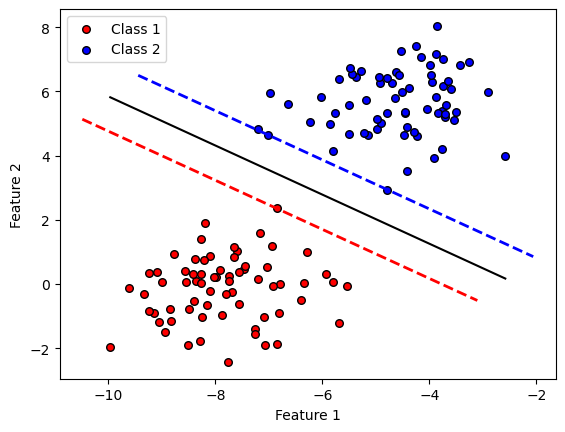
\includegraphics[width=\textwidth]{images/classicalsvm.png}
    \caption{SVM decision boundary and margin border, fitted on a 2 feature mock dataset of 100 istances.}
    \label{fig:classical svm mock}
\end{figure}

We now need to address the issue of dealing with a highly non-linearly separable dataset. Let's consider as an example another mock dataset, shown in Figure (\ref{fig:classical svm circles}). 
\begin{figure}[h!]
    \centering
    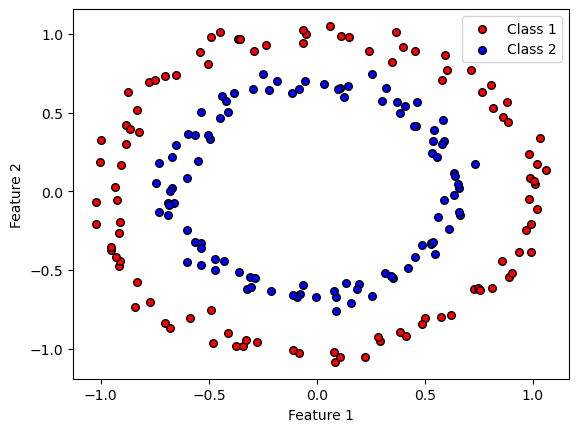
\includegraphics[width=\textwidth]{images/circles.png}
    \caption{Higly non-linear 2 feature mock dataset with 100 istances.}
    \label{fig:classical svm circles}
\end{figure}
It is clear that in this case we cannot use the SVM alghoritm in its basic form, not even with a soft margin. We must introduce the idea of kernelization. 
Let's introduce a function, called feature map, which projects the data in a higher dimensional space. That means a function
\begin{equation}
    \phi:\mathbb{R}^d\rightarrow\mathbb{R}^D,
\end{equation}
with $D>d$. If we choose a suitable feature map we can hope to obtain a linearly separable dataset in the higher dimensional space. The choice of the feature map is completely arbitrary, as long as it is a bijective function. Therefore, in principle, each time we are given a dataset we must choose an appropriate feature map for this strategy to work. For our example let's consider the feature map
$$    \phi:\mathbb{R}^2\rightarrow\mathbb{R}^3,$$
\begin{equation}
    \begin{pmatrix}
        x_0\\
        x_1
        \end{pmatrix} \mapsto  
        \begin{pmatrix}
        x_0^2 \\
        x_1^2\\
        x_0^2+x_1^2
        \end{pmatrix} .
\end{equation}
The data of Figure (\ref{fig:classical svm circles}) after the application of the feature map $\phi$ are represented in Figure (\ref{fig:classical svm circle 3d}). 
\begin{figure}[h!]
    \centering
    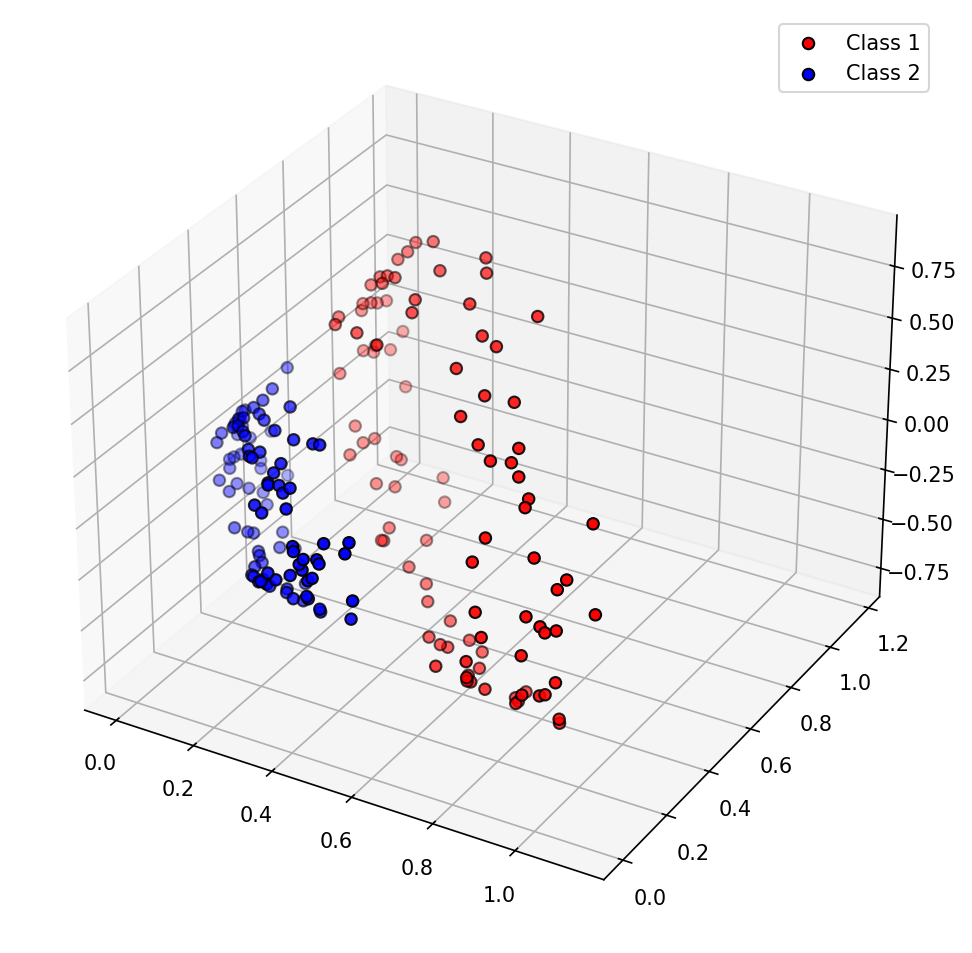
\includegraphics[width=\textwidth]{images/circles3d.png}
    \caption{Higly non-linear mock dataset after the application of the feature map $\phi$. We observe now that the dataset is linearly separable.}
    \label{fig:classical svm circle 3d}
\end{figure}
The dataset is now linearly separable in the higher dimensional space, so the strategy worked. We can now apply the SVM alghoritm in this space Consider the two central equations of the algorithm: equation (\ref{dual problem SVM}), which provides the expression to maximize in order to find the margin, and equation (\ref{decision boundary svm}), which gives the rule for predicting the class of a new instance. This two equations are now modified into 
\begin{equation}
    f(\alpha_0,\cdots,\alpha_{N-1})=\sum_{i=0}^{N-1} \alpha_i-\frac{1}{2}\sum_{i=0}^{N-1}\sum_{j=0}^{N-1}\alpha_i\alpha_jy_iy_j(\phi(\mathbf{x}_i,)\phi(\mathbf{x}_j)),
    \label{kernel max}
\end{equation}
\begin{equation}
    \textup{sign}\left[\sum_{i=0}^{N-1}\alpha_iy_i(\phi(\mathbf{\tilde{x}}), \phi(\mathbf{x}_i))+w_0\right].
    \label{kernel prodiction}
\end{equation}
A crucial observation is that in these two expressions only the scalar product of the feature map values appears. Therefore we can conclude that the specific form of the feature map is not important, but rather the scalar product it produces. We can define the kernel $K$ as 
$$K:\mathbb{R}^d\times \mathbb{R}^d\rightarrow \mathbb{R},$$
\begin{equation}
    (\mathbf{x}, \mathbf{y})\mapsto(\phi(\mathbf{x}), \phi(\mathbf{y})),
\end{equation}
 where $(\phi(\mathbf{x}), \phi(\mathbf{y}))=\phi(\mathbf{x})^T\cdot \phi(\mathbf{y})$ is the standard scalar product of $\mathbb{R}^D$. Eq. (\ref{kernel max}) and eq. (\ref{kernel prodiction}) now become 
 \begin{equation}
    f(\alpha_0,\cdots,\alpha_{N-1})=\sum_{i=0}^{N-1} \alpha_i-\frac{1}{2}\sum_{i=0}^{N-1}\sum_{j=0}^{N-1}\alpha_i\alpha_jy_iy_jK(\mathbf{x}_i,\mathbf{x}_j),
    \label{kernel max K}
\end{equation}
\begin{equation}
    \textup{sign}\left[\sum_{i=0}^{N-1}\alpha_iy_iK(\mathbf{\tilde{x}}, \mathbf{x}_i)+w_0\right].
    \label{kernel prodiction K}
\end{equation}
We see explicitly that the only quantity that matters is the kernel $K$. In our specific example the value of the kernel is 











\end{document}